\hypertarget{major-diseases-of-the-nervous-system}{%
\chapter{Major Diseases Of The Nervous
System}\label{major-diseases-of-the-nervous-system}}

\hypertarget{neurodegenerative-diseases}{%
\section{Neurodegenerative
Diseases}\label{neurodegenerative-diseases}}

Neurodegeneration is the progressive loss of structure or function of
neurons, including death of neurons. Many neurodegenerative diseases --
including amyotrophic lateral sclerosis, Parkinson's disease,
Alzheimer's disease, fatal familial insomnia, and Huntington's disease
-- occur as a result of neurodegenerative processes. Such diseases are
incurable, resulting in progressive degeneration and/or death of
neurons. As research progresses, many similarities appear that relate
these diseases to one another on a sub-cellular level. Discovering these
similarities offers hope for therapeutic advances that could ameliorate
many diseases simultaneously. There are many parallels between different
neurodegenerative disorders including atypical protein assemblies as
well as induced cell death. Neurodegeneration can be found in many
different levels of neuronal circuitry ranging from molecular to
systemic.

The greatest risk factor for neurodegenerative diseases is aging.
Mitochondrial DNA mutations as well as oxidative stress both contribute
to aging. Many of these diseases are late-onset, meaning there is some
factor that changes as a person ages for each disease. One constant
factor is that in each disease, neurons gradually lose function as the
disease progresses with age. It has been proposed that DNA damage
accumulation provides the underlying causative link between aging and
neurodegenerative disease. About 20-40\% of healthy people between 60
and 78 years old experience discernable decrements in cognitive
performance in several domains including working, spatial, and episodic
memory, and processing speed.

Many neurodegenerative diseases are caused by genetic mutations, most of
which are located in completely unrelated genes. In many of the
different diseases, the mutated gene has a common feature: a repeat of
the CAG nucleotide triplet. CAG codes for the amino acid glutamine. A
repeat of CAG results in a polyglutamine (polyQ) tract. Diseases
associated with such mutations are known as trinucleotide repeat
disorders.

Polyglutamine repeats typically cause dominant pathogenesis. Extra
glutamine residues can acquire toxic properties through a variety of
ways, including irregular protein folding and degradation pathways,
altered subcellular localization, and abnormal interactions with other
cellular proteins. PolyQ studies often use a variety of animal models
because there is such a clearly defined trigger -- repeat expansion.
Extensive research has been done using the models of nematode (C.
elegans), and fruit fly (Drosophila), mice, and non-human primates.

Nine inherited neurodegenerative diseases are caused by the expansion of
the CAG trinucleotide and polyQ tract, including Huntington's disease
and the spinocerebellar ataxias.

Several neurodegenerative diseases are classified as proteopathies as
they are associated with the aggregation of misfolded proteins.

\begin{itemize}
\tightlist
\item
  alpha-synuclein: can aggregate to form insoluble fibrils in
  pathological conditions characterized by Lewy bodies, such as
  Parkinson's disease, dementia with Lewy bodies, and multiple system
  atrophy. Alpha-synuclein is the primary structural component of Lewy
  body fibrils. In addition, an alpha-synuclein fragment, known as the
  non-Abeta component (NAC), is found in amyloid plaques in Alzheimer's
  disease.
\item
  tau: hyperphosphorylated tau protein is the main component of
  neurofibrillary tangles in Alzheimer's disease.
\item
  beta amyloid: the major component of senile plaques in Alzheimer's
  disease.
\item
  prion: main component of prion diseases and transmissible spongiform
  encephalopathies.
\end{itemize}

\hypertarget{alzheimers-disease}{%
\subsubsection{Alzheimer's disease}\label{alzheimers-disease}}

Alzheimer's disease (AD) is a chronic neurodegenerative disease that
results in the loss of neurons and synapses in the cerebral cortex and
certain subcortical structures, resulting in gross atrophy of the
temporal lobe, parietal lobe, and parts of the frontal cortex and
cingulate gyrus.

\begin{figure}

{\centering 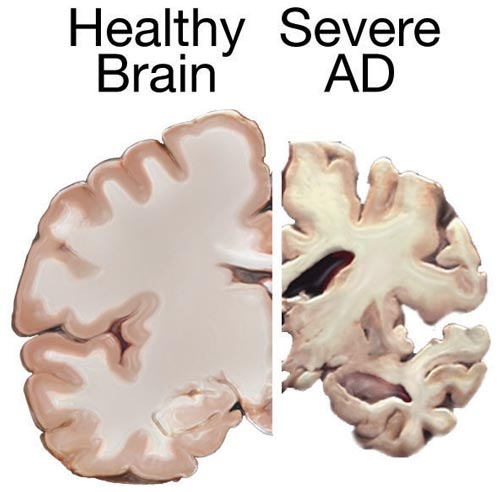
\includegraphics[width=0.7\linewidth]{./figures/disease/Alzheimers_brain} 

}

\caption{Comparison of brain tissue between healthy individual and Alzheimer's disease patient, demonstrating extent of neuronal death \href{https://commons.wikimedia.org/wiki/File:Alzheimers_brain.jpg} }\label{fig:alzheimerbrain}

\end{figure}

AD pathology is primarily characterized by the presence of senile
plaques and neurofibrillary tangles. Plaques are made up of small
peptides, typically 39--43 amino acids in length, called beta-amyloid
(also written as A-beta or Aβ). Beta-amyloid is a fragment from a larger
protein called amyloid precursor protein (APP), a transmembrane protein
that penetrates through the neuron's membrane. APP appears to play roles
in normal neuron growth, survival and post-injury repair. APP is cleaved
into smaller fragments by enzymes such as gamma secretase and beta
secretase. One of these fragments gives rise to fibrils of beta-amyloid
which can self-assemble into the dense extracellular deposits known as
senile plaques or amyloid plaques.

\begin{figure}

{\centering 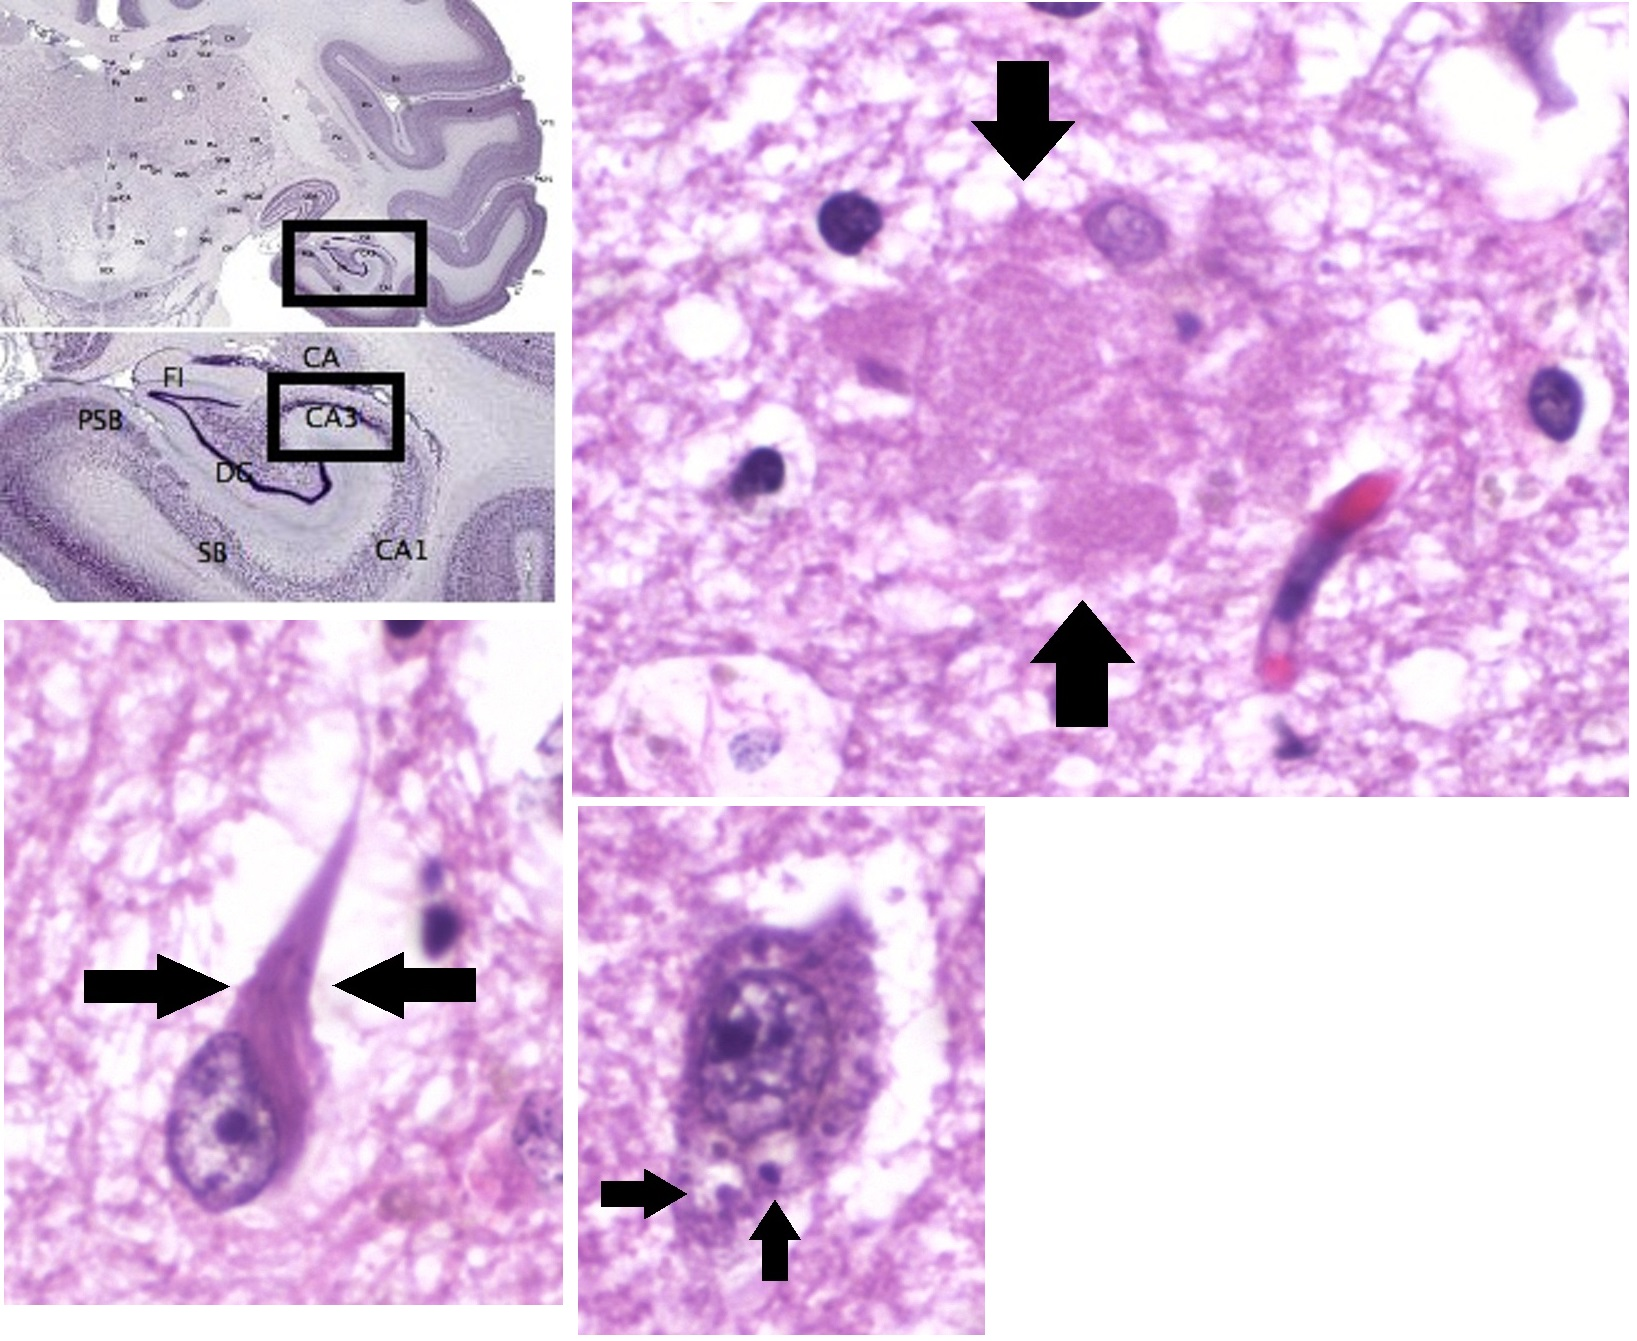
\includegraphics[width=0.7\linewidth]{./figures/disease/Histopathology_of_Alzheimer's_disease} 

}

\caption{Histopathologic images of Alzheimer's disease, in the CA3 area of the hippocampus, showing an amyloid plaque (top right), neurofibrillary tangles (bottom left) and granulovacuolar degeneration (bottom center). \href{https://commons.wikimedia.org/wiki/File:Histopathology_of_Alzheimer\%27s_disease.jpg}} \label{fig:alzheimer}

\end{figure}

\hypertarget{parkinsons-disease}{%
\subsubsection{Parkinson's disease}\label{parkinsons-disease}}

Parkinson's disease (PD) is the second most common neurodegenerative
disorder. It typically manifests as bradykinesia, rigidity, resting
tremor and posture instability. The crude prevalence rate of PD has been
reported to range from 15 per 100,000 to 12,500 per 100,000, and the
incidence of PD from 15 per 100,000 to 328 per 100,000, with the disease
being less common in Asian countries.

PD is primarily characterized by death of dopaminergic neurons in the
substantia nigra, a region of the midbrain. The cause of this selective
cell death is unknown. Notably, alpha-synuclein-ubiquitin complexes and
aggregates are observed to accumulate in Lewy bodies within affected
neurons. It is thought that defects in protein transport machinery and
regulation, such as RAB1, may play a role in this disease mechanism.
Impaired axonal transport of alpha-synuclein may also lead to its
accumulation in Lewy bodies. Experiments have revealed reduced transport
rates of both wild-type and two familial Parkinson's disease-associated
mutant alpha-synucleins through axons of cultured neurons. Membrane
damage by alpha-synuclein could be another Parkinson's disease
mechanism.

\begin{figure}

{\centering 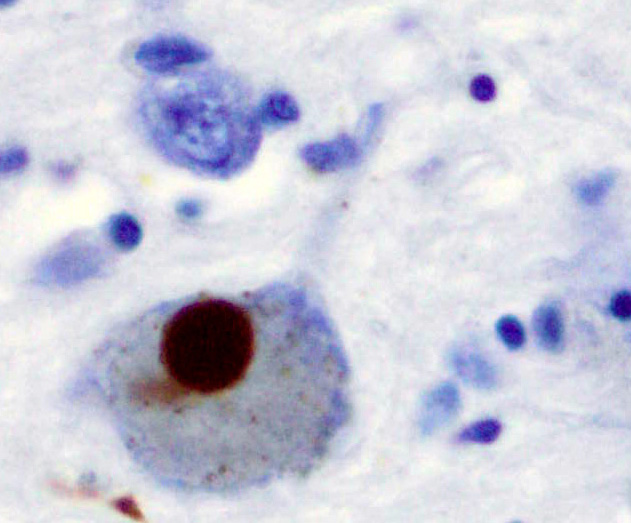
\includegraphics[width=0.7\linewidth]{./figures/disease/Lewy_Body_alphaSynuclein} 

}

\caption{A Lewy body (stained brown) in a brain cell of the substantia nigra in Parkinson's disease. The brown colour is positive immunohistochemistry staining for alpha-synuclein.\href{https://commons.wikimedia.org/wiki/File:Lewy_Body_alphaSynuclein.jpg}} \label{fig:parkinson} 

\end{figure}


The main known risk factor is age. Mutations in genes such as
α-synuclein (SNCA), leucine-rich repeat kinase 2 (LRRK2),
glucocerebrosidase (GBA), and tau protein (MAPT) can also cause
hereditary PD or increase PD risk.

\hypertarget{huntingtons-disease}{%
\subsubsection{Huntington's disease}\label{huntingtons-disease}}

Huntington's disease (HD) is a rare autosomal dominant neurodegenerative
disorder caused by mutations in the huntingtin gene. HD is characterized
by loss of medium spiny neurons and astrogliosis. The first brain region
to be substantially affected is the striatum, followed by degeneration
of the frontal and temporal cortices. The striatum's subthalamic nuclei
send control signals to the globus pallidus, which initiates and
modulates motion. The weaker signals from subthalamic nuclei thus cause
reduced initiation and modulation of movement, resulting in the
characteristic movements of the disorder, notably chorea.

HD is caused by polyglutamine tract expansion in the huntingtin gene,
resulting in the aggregation-prone mutant huntingtin (mHtt). mHtt
aggregates may be directly toxic. Additionally, they may damage
molecular motors and microtubules to interfere with normal axonal
transport, leading to impaired transport of important cargoes such as
BDNF.

\hypertarget{amyotrophic-lateral-sclerosis-als}{%
\subsubsection{Amyotrophic lateral sclerosis
(ALS)}\label{amyotrophic-lateral-sclerosis-als}}

Amyotrophic lateral sclerosis (ALS or Lou Gehrig's disease) is a disease
in which motor neurons are selectively targeted for degeneration. In
1993, missense mutations in the gene encoding the antioxidant enzyme
Cu/Zn superoxide dismutase 1 (SOD1) were discovered in a subsets of
patients with familial ALS. This discovery led researchers to focus on
unlocking the mechanisms for SOD1-mediated diseases. However, the
pathogenic mechanism underlying SOD1 mutant toxicity has yet to be
resolved. More recently, TDP-43 and FUS protein aggregates have been
implicated in some cases of the disease, and a mutation in chromosome 9
(C9orf72) is thought to be the most common known cause of sporadic ALS.

Recent independent research by Nagai et al.~and Di Giorgio et
al.~provide in vitro evidence that the primary cellular sites where SOD1
mutations act are located on astrocytes. Astrocytes then cause the toxic
effects on the motor neurons. The specific mechanism of toxicity still
needs to be investigated, but the findings are significant because they
implicate cells other than neuron cells in neurodegeneration.

\hypertarget{cerebrovascular-disease}{%
\section{Cerebrovascular Disease}\label{cerebrovascular-disease}}

Cerebrovascular disease includes a variety of medical conditions that
affect the blood vessels of the brain and the cerebral circulation.
Arteries supplying oxygen and nutrients to the brain are often damaged
or deformed in these disorders. The most common presentation of
cerebrovascular disease is an ischemic stroke or mini-stroke and
sometimes a hemorrhagic stroke. Hypertension (high blood pressure) is
the most important contributing risk factor for stroke and
cerebrovascular diseases as it can change the structure of blood vessels
and result in atherosclerosis. Atherosclerosis narrows blood vessels in
the brain, resulting in decreased cerebral perfusion. Other risk factors
that contribute to stroke include smoking and diabetes. Narrowed
cerebral arteries can lead to ischemic stroke, but continually elevated
blood pressure can also cause tearing of vessels, leading to a
hemorrhagic stroke.

\hypertarget{stroke}{%
\subsubsection{Stroke}\label{stroke}}

A stroke is a medical condition in which poor blood flow to the brain
causes cell death. There are two main types of stroke: ischemic, due to
lack of blood flow, and hemorrhagic, due to bleeding. Both cause parts
of the brain to stop functioning properly. Signs and symptoms of a
stroke may include an inability to move or feel on one side of the body,
problems understanding or speaking, dizziness, or loss of vision to one
side. Signs and symptoms often appear soon after the stroke has
occurred. If symptoms last less than one or two hours, the stroke is a
transient ischemic attack (TIA), also called a mini-stroke. A
hemorrhagic stroke may also be associated with a severe headache. The
symptoms of a stroke can be permanent. Long-term complications may
include pneumonia and loss of bladder control.

\begin{figure}

{\centering 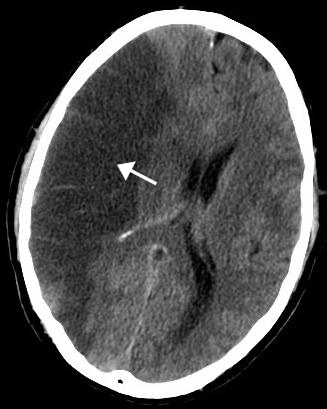
\includegraphics[width=0.7\linewidth]{./figures/disease/MCA_Territory_Infarct} 

}

\caption{CT-scan
of the brain with an MCA infarct.\href{https://commons.wikimedia.org/wiki/File:MCA_Territory_Infarct.svg} } \label{fig:ctstroke}

\end{figure}

The main risk factor for stroke is high blood pressure. Other risk
factors include tobacco smoking, obesity, high blood cholesterol,
diabetes mellitus, a previous TIA, end-stage kidney disease, and atrial
fibrillation. An ischemic stroke is typically caused by blockage of a
blood vessel, though there are also less common causes. A hemorrhagic
stroke is caused by either bleeding directly into the brain or into the
space between the brain's membranes. Bleeding may occur due to a
ruptured brain aneurysm. Diagnosis is typically based on a physical exam
and supported by medical imaging such as a CT scan or MRI scan. A CT
scan can rule out bleeding, but may not necessarily rule out ischemia,
which early on typically does not show up on a CT scan. Other tests such
as an electrocardiogram (ECG) and blood tests are done to determine risk
factors and rule out other possible causes. Low blood sugar may cause
similar symptoms.

Prevention includes decreasing risk factors, surgery to open up the
arteries to the brain in those with problematic carotid narrowing, and
warfarin in people with atrial fibrillation. Aspirin or statins may be
recommended by physicians for prevention. A stroke or TIA often requires
emergency care. An ischemic stroke, if detected within three to four and
half hours, may be treatable with a medication that can break down the
clot. Some hemorrhagic strokes benefit from surgery. Treatment to
attempt recovery of lost function is called stroke rehabilitation, and
ideally takes place in a stroke unit; however, these are not available
in much of the world.

In 2013, approximately 6.9 million people had an ischemic stroke and 3.4
million people had a hemorrhagic stroke. In 2015, there were about 42.4
million people who had previously had a stroke and were still alive.
Between 1990 and 2010 the number of strokes which occurred each year
decreased by approximately 10\% in the developed world and increased by
10\% in the developing world. In 2015, stroke was the second most
frequent cause of death after coronary artery disease, accounting for
6.3 million deaths (11\% of the total). About 3.0 million deaths
resulted from ischemic stroke while 3.3 million deaths resulted from
hemorrhagic stroke. About half of people who have had a stroke live less
than one year. Overall, two thirds of strokes occurred in those over 65
years old.

Strokes can be classified into two major categories: ischemic and
hemorrhagic. Ischemic strokes are caused by interruption of the blood
supply to the brain, while hemorrhagic strokes result from the rupture
of a blood vessel or an abnormal vascular structure. About 87\% of
strokes are ischemic, the rest being hemorrhagic. Bleeding can develop
inside areas of ischemia, a condition known as ``hemorrhagic
transformation.'' It is unknown how many hemorrhagic strokes actually
start as ischemic strokes.

In the 1970s the World Health Organization defined stroke as a
``neurological deficit of cerebrovascular cause that persists beyond 24
hours or is interrupted by death within 24 hours'', although the word
``stroke'' is centuries old. This definition was supposed to reflect the
reversibility of tissue damage and was devised for the purpose, with the
time frame of 24 hours being chosen arbitrarily. The 24-hour limit
divides stroke from transient ischemic attack, which is a related
syndrome of stroke symptoms that resolve completely within 24 hours.
With the availability of treatments that can reduce stroke severity when
given early, many now prefer alternative terminology, such as brain
attack and acute ischemic cerebrovascular syndrome (modeled after heart
attack and acute coronary syndrome, respectively), to reflect the
urgency of stroke symptoms and the need to act swiftly.

In an ischemic stroke, blood supply to part of the brain is decreased,
leading to dysfunction of the brain tissue in that area. There are four
reasons why this might happen:

\begin{itemize}
\tightlist
\item
  Thrombosis (obstruction of a blood vessel by a blood clot forming
  locally)
\item
  Embolism (obstruction due to an embolus from elsewhere in the body),
\item
  Systemic hypoperfusion (general decrease in blood supply, e.g., in
  shock)
\item
  Cerebral venous sinus thrombosis.
\end{itemize}

There are various classification systems for acute ischemic stroke. The
Oxford Community Stroke Project classification (OCSP, also known as the
Bamford or Oxford classification) relies primarily on the initial
symptoms; based on the extent of the symptoms, the stroke episode is
classified as total anterior circulation infarct (TACI), partial
anterior circulation infarct (PACI), lacunar infarct (LACI) or posterior
circulation infarct (POCI). These four entities predict the extent of
the stroke, the area of the brain that is affected, the underlying
cause, and the prognosis. The TOAST (Trial of Org 10172 in Acute Stroke
Treatment) classification is based on clinical symptoms as well as
results of further investigations; on this basis, a stroke is classified
as being due to (1) thrombosis or embolism due to atherosclerosis of a
large artery, (2) an embolism originating in the heart, (3) complete
blockage of a small blood vessel, (4) other determined cause, (5)
undetermined cause (two possible causes, no cause identified, or
incomplete investigation). Users of stimulants such as cocaine and
methamphetamine are at a high risk for ischemic strokes.

There are two main types of hemorrhagic stroke:

\begin{itemize}
\tightlist
\item
  Intracerebral hemorrhage, which is basically bleeding within the brain
  itself (when an artery in the brain bursts, flooding the surrounding
  tissue with blood), due to either intraparenchymal hemorrhage
  (bleeding within the brain tissue) or intraventricular hemorrhage
  (bleeding within the brain's ventricular system).
\item
  Subarachnoid hemorrhage, which is basically bleeding that occurs
  outside of the brain tissue but still within the skull, and precisely
  between the arachnoid mater and pia mater (the delicate innermost
  layer of the three layers of the meninges that surround the brain).
\end{itemize}

The above two main types of hemorrhagic stroke are also two different
forms of intracranial hemorrhage, which is the accumulation of blood
anywhere within the cranial vault; but the other forms of intracranial
hemorrhage, such as epidural hematoma (bleeding between the skull and
the dura mater, which is the thick outermost layer of the meninges that
surround the brain) and subdural hematoma (bleeding in the subdural
space), are not considered ``hemorrhagic strokes''.

Hemorrhagic strokes may occur on the background of alterations to the
blood vessels in the brain, such as cerebral amyloid angiopathy,
cerebral arteriovenous malformation and an intracranial aneurysm, which
can cause intraparenchymal or subarachnoid hemorrhage.

In addition to neurological impairment, hemorrhagic strokes usually
cause specific symptoms (for instance, subarachnoid hemorrhage
classically causes a severe headache known as a thunderclap headache) or
reveal evidence of a previous head injury.

Stroke symptoms typically start suddenly, over seconds to minutes, and
in most cases do not progress further. The symptoms depend on the area
of the brain affected. The more extensive the area of the brain
affected, the more functions that are likely to be lost.

\hypertarget{aphasia}{%
\subsubsection{Aphasia}\label{aphasia}}

Aphasia is an inability to comprehend or formulate language because of
damage to specific brain regions. Aphasia is most often caused by
stroke, but any disease or damage to the parts of the brain that control
language can cause aphasia. Some of these can include brain tumors,
traumatic brain injury, and progressive neurological disorders.

People with aphasia may experience any of the following behaviors due to
an acquired brain injury, although some of these symptoms may be due to
related or concomitant problems, such as dysarthria or apraxia, and not
primarily due to aphasia. Aphasia symptoms can vary based on the
location of damage in the brain. Signs and symptoms may or may not be
present in individuals with aphasia and may vary in severity and level
of disruption to communication. Often those with aphasia will try to
hide their inability to name objects by using words like thing. So when
asked to name a pencil they may say it is a thing used to write.

\begin{itemize}
\item
  Inability to comprehend language
\item
  Inability to pronounce, not due to muscle paralysis or weakness
\item
  Inability to speak spontaneously
\item
  Inability to form words
\item
  Inability to name objects (anomia)
\item
  Poor enunciation
\item
  Excessive creation and use of personal neologisms
\item
  Inability to repeat a phrase
\item
  Persistent repetition of one syllable, word, or phrase (stereotypies,
  recurrent/recurring utterances/speech automatism)
\item
  Paraphasia (substituting letters, syllables or words)
\item
  Agrammatism (inability to speak in a grammatically correct fashion)
\item
  Dysprosody (alterations in inflexion, stress, and rhythm)
\item
  Incomplete sentences
\item
  Inability to read
\item
  Inability to write
\item
  Limited verbal output
\item
  Difficulty in naming
\item
  Speech disorder
\item
  Speaking gibberish
\item
  Inability to follow or understand simple requests
\end{itemize}

Localizationist approaches aim to classify the aphasias according to
their major presenting characteristics and the regions of the brain that
most probably gave rise to them. Inspired by the early work of
nineteenth-century neurologists \href{}{Paul Broca} and \href{}{Carl
Wernicke}, these approaches identify two major subtypes of aphasia and
several more minor subtypes:

\begin{figure}

{\centering 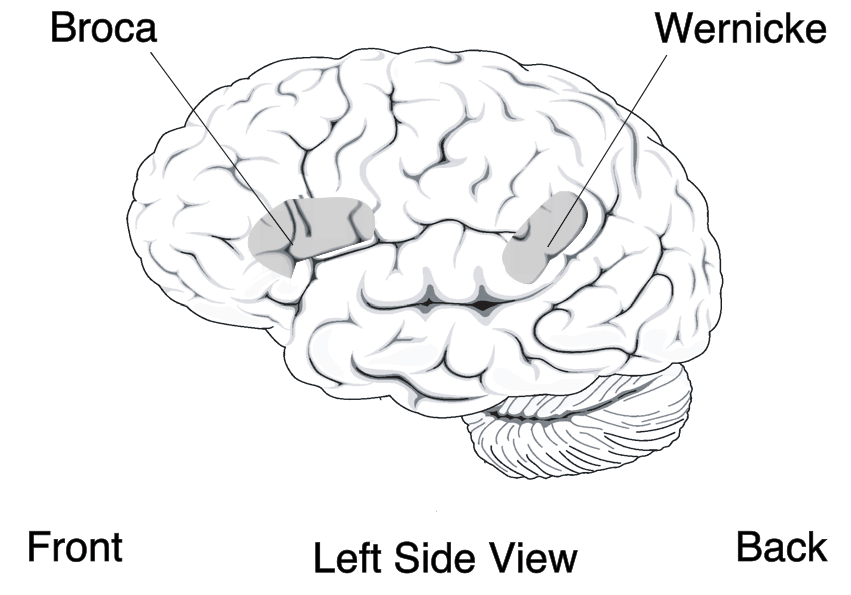
\includegraphics[width=0.7\linewidth]{./figures/disease/BrocasAreaSmall} 

}

\caption{Cortical areas damaged in Broaca's and Wernicke's aphasia.\href{https://commons.wikimedia.org/wiki/File:BrocasAreaSmall.png}}\label{fig:aphasias}

\end{figure}

\begin{itemize}
\tightlist
\item
  Expressive aphasia (also known as ``motor aphasia'' or ``Broca's
  aphasia''), which is characterized by halted, fragmented, effortful
  speech, but well-preserved comprehension relative to expression.
  Damage is typically in the anterior portion of the left hemisphere,
  most notably Broca's area. Individuals with Broca's aphasia often have
  right-sided weakness or paralysis of the arm and leg, because the left
  frontal lobe is also important for body movement, particularly on the
  right side.
\item
  Receptive aphasia (also known as ``sensory aphasia'' or ``Wernicke's
  aphasia''), which is characterized by fluent speech, but marked
  difficulties understanding words and sentences. Although fluent, the
  speech may lack in key substantive words (nouns, verbs, adjectives),
  and may contain incorrect words or even nonsense words. This subtype
  has been associated with damage to the posterior left temporal cortex,
  most notably Wernicke's area. These individuals usually have no body
  weakness, because their brain injury is not near the parts of the
  brain that control movement.
\item
  Conduction aphasia, where speech remains fluent, and comprehension is
  preserved, but the person may have disproportionate difficulty where
  repeating words or sentences. Damage typically involves the arcuate
  fasciculus and the left parietal region.
\item
  Transcortical motor aphasia and transcortical sensory aphasia, which
  are similar to Broca's and Wernicke's aphasia respectively, but the
  ability to repeat words and sentences is disproportionately preserved.
\end{itemize}

Recent classification schemes adopting this approach, such as the
Boston-Neoclassical Model, also group these classical aphasia subtypes
into two larger classes: the nonfluent aphasias (which encompasses
Broca's aphasia and transcortical motor aphasia) and the fluent aphasias
(which encompasses Wernicke's aphasia, conduction aphasia and
transcortical sensory aphasia). These schemes also identify several
further aphasia subtypes, including: anomic aphasia, which is
characterized by a selective difficulty finding the names for things;
and global aphasia, where both expression and comprehension of speech
are severely compromised.

Many localizationist approaches also recognize the existence of
additional, more ``pure'' forms of language disorder that may affect
only a single language skill. For example, in pure alexia, a person may
be able to write but not read, and in pure word deafness, they may be
able to produce speech and to read, but not understand speech when it is
spoken to them.

\hypertarget{prosopagnosia}{%
\subsubsection{Prosopagnosia}\label{prosopagnosia}}

Prosopagnosia (from Greek prósōpon, meaning ``face'', and agnōsía,
meaning ``non-knowledge''), also called face blindness, is a cognitive
disorder of face perception in which the ability to recognize familiar
faces, including one's own face (self-recognition), is impaired, while
other aspects of visual processing (e.g., object discrimination) and
intellectual functioning (e.g., decision-making) remain intact. The term
originally referred to a condition following acute brain damage
(acquired prosopagnosia), but a congenital or developmental form of the
disorder also exists, with a prevalence rate of 2.5\%. The specific
brain area usually associated with prosopagnosia is the fusiform gyrus,
which activates specifically in response to faces. The functionality of
the fusiform gyrus allows most people to recognize faces in more detail
than they do similarly complex inanimate objects. For those with
prosopagnosia, the new method for recognizing faces depends on the less
sensitive object-recognition system. The right hemisphere fusiform gyrus
is more often involved in familiar face recognition than the left. It
remains unclear whether the fusiform gyrus is only specific for the
recognition of human faces or if it is also involved in highly trained
visual stimuli.

Acquired prosopagnosia results from occipito-temporal lobe damage and is
most often found in adults. This is further subdivided into apperceptive
and associative prosopagnosia. In congenital prosopagnosia, the
individual never adequately develops the ability to recognize faces.

Though there have been several attempts at remediation, no therapies
have demonstrated lasting real-world improvements across a group of
prosopagnosics. Prosopagnosics often learn to use ``piecemeal'' or
``feature-by-feature'' recognition strategies. This may involve
secondary clues such as clothing, gait, hair color, skin color, body
shape, and voice. Because the face seems to function as an important
identifying feature in memory, it can also be difficult for people with
this condition to keep track of information about people, and socialize
normally with others. Prosopagnosia has also been associated with other
disorders that are associated with nearby brain areas: left hemianopsia
(loss of vision from left side of space, associated with damage to the
right occipital lobe), achromatopsia (a deficit in color perception
often associated with unilateral or bilateral lesions in the
temporo-occipital junction) and topographical disorientation (a loss of
environmental familiarity and difficulties in using landmarks,
associated with lesions in the posterior part of the parahippocampal
gyrus and anterior part of the lingual gyrus of the right hemisphere).

\hypertarget{hemispatial-neglect}{%
\subsubsection{Hemispatial neglect}\label{hemispatial-neglect}}

Hemispatial neglect is a neuropsychological condition in which, after
damage to one hemisphere of the brain is sustained, a deficit in
attention to and awareness of one side of the field of vision is
observed. It is defined by the inability of a person to process and
perceive stimuli on one side of the body or environment, where that
inability is not due to a lack of sensation. Hemispatial neglect is very
commonly contralateral to the damaged hemisphere, but instances of
ipsilesional neglect (on the same side as the lesion) have been
reported.

Hemispatial neglect results most commonly from strokes and brain
unilateral injury to the right cerebral hemisphere, with rates in the
critical stage of up to 80\% causing visual neglect of the left-hand
side of space. Neglect is often produced by massive strokes in the
middle cerebral artery region and is variegated, so that most sufferers
do not exhibit all of the syndrome's traits. Right-sided spatial neglect
is rare because there is redundant processing of the right space by both
the left and right cerebral hemispheres, whereas in most left-dominant
brains the left space is only processed by the right cerebral
hemisphere. Although it most strikingly affects visual perception
(`visual neglect'), neglect in other forms of perception can also be
found, either alone or in combination with visual neglect.

For example, a stroke affecting the right parietal lobe of the brain can
lead to neglect for the left side of the visual field, causing a patient
with neglect to behave as if the left side of sensory space is
nonexistent (although they can still turn left). In an extreme case, a
patient with neglect might fail to eat the food on the left half of
their plate, even though they complain of being hungry. If someone with
neglect is asked to draw a clock, their drawing might show only the
numbers 12 to 6, or all 12 numbers might be on one half of the clock
face with the other half distorted or blank. Neglect patients may also
ignore the contralesional side of their body; for instance, they might
only shave, or apply make-up to, the non-neglected side. These patients
may frequently collide with objects or structures such as door frames on
the side being neglected.

Neglect may also present as a delusional form, where the patient denies
ownership of a limb or an entire side of the body. Since this delusion
often occurs alone, without the accompaniment of other delusions, it is
often labeled as a monothematic delusion.

Neglect not only affects present sensation but memory and recall
perception as well. A patient suffering from neglect may also, when
asked to recall a memory of a certain object and then draw said object,
draw only half of the object. It is unclear, however, if this is due to
a perceptive deficit of the memory (to the patient having lost pieces of
spatial information of the memory) or whether the information within the
memory is whole and intact but simply being ignored, the same way
portions of a physical object in the patient's presence would be
ignored.

Some forms of neglect may also be very mild---for example, in a
condition called extinction where competition from the ipsilesional
stimulus impedes perception of the contralesional stimulus. These
patients, when asked to fixate on the examiner's nose, can detect
fingers being wiggled on the affected side. If the examiner were to
wiggle his or her fingers on both the affected and unaffected sides of
the patient, the patient will report seeing movement only on the
ipsilesional side.

\hypertarget{epilepsy}{%
\section{Epilepsy}\label{epilepsy}}

Epilepsy is a group of neurological disorders characterized by recurrent
epileptic seizures. Epileptic seizures are episodes that can vary from
brief and nearly undetectable periods to long periods of vigorous
shaking. These episodes can result in physical injuries, including
occasionally broken bones. In epilepsy, seizures have a tendency to
recur and, as a rule, have no immediate underlying cause. Isolated
seizures that are provoked by a specific cause such as poisoning are not
deemed to represent epilepsy. People with epilepsy may be treated
differently in various areas of the world and experience varying degrees
of social stigma due to their condition.

\begin{figure}

{\centering 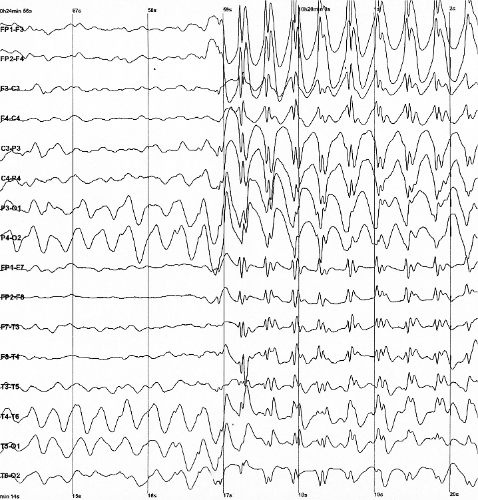
\includegraphics[width=0.7\linewidth]{./figures/disease/Spike-waves} 

}

\caption{The electroencephalogram recording of a person with childhood absence epilepsy showing a seizure. \href{https://commons.wikimedia.org/wiki/File:Spike-waves.png} The waves are black on a white background.}\label{fig:epilepsyeeg}

\end{figure}

The underlying mechanism of epileptic seizures is excessive and abnormal
neuronal activity in the cortex of the brain. The reason this occurs in
most cases of epilepsy is unknown. Some cases occur as the result of
brain injury, stroke, brain tumors, infections of the brain, or birth
defects through a process known as epileptogenesis. Known genetic
mutations are directly linked to a small proportion of cases. The
diagnosis involves ruling out other conditions that might cause similar
symptoms, such as fainting, and determining if another cause of seizures
is present, such as alcohol withdrawal or electrolyte problems. This may
be partly done by imaging the brain and performing blood tests. Epilepsy
can often be confirmed with an electroencephalogram (EEG), but a normal
test does not rule out the condition.

Epilepsy that occurs as a result of other issues may be preventable.
Seizures are controllable with medication in about 70\% of cases;
inexpensive anti-seizure medications are often available. In those whose
seizures do not respond to medication, surgery, neurostimulation or
dietary changes may then be considered. Not all cases of epilepsy are
lifelong, and many people improve to the point that treatment is no
longer needed.

As of 2015, about 39 million people have epilepsy. Nearly 80\% of cases
occur in the developing world. In 2015, it resulted in 125,000 deaths,
an increase from 112,000 in 1990. Epilepsy is more common in older
people. In the developed world, onset of new cases occurs most
frequently in babies and the elderly. In the developing world, onset is
more common in older children and young adults due to differences in the
frequency of the underlying causes. About 5--10\% of people will have an
unprovoked seizure by the age of 80, and the chance of experiencing a
second seizure is between 40\% and 50\%. In many areas of the world,
those with epilepsy either have restrictions placed on their ability to
drive or are not permitted to drive until they are free of seizures for
a specific length of time. The word epilepsy is from Ancient Greek
ἐπιλαμβάνειν, `to seize, possess, or afflict'.

Normally brain electrical activity is non-synchronous, as neurons do not
normally fire in sync with each other, but rather fire in order as
signals travel throughout the brain. Its activity is regulated by
various factors both within the neuron and the cellular environment.
Factors within the neuron include the type, number and distribution of
ion channels, changes to receptors and changes of gene expression.
Factors around the neuron include ion concentrations, synaptic
plasticity and regulation of transmitter breakdown by glial cells.
Chronic inflammation also appears to play a role.

The exact mechanism of epilepsy is unknown, but a little is known about
its cellular and network mechanisms. However, it is unknown under which
circumstances the brain shifts into the activity of a seizure with its
excessive synchronization.

In epilepsy, the resistance of excitatory neurons to fire during this
period is decreased. This may occur due to changes in ion channels or
inhibitory neurons not functioning properly. This then results in a
specific area from which seizures may develop, known as a ``seizure
focus''. Another mechanism of epilepsy may be the up-regulation of
excitatory circuits or down-regulation of inhibitory circuits following
an injury to the brain. These secondary epilepsies occur through
processes known as epileptogenesis. Failure of the blood--brain barrier
may also be a causal mechanism as it would allow substances in the blood
to enter the brain.

There is evidence that epileptic seizures are usually not a random
event. Seizures are often brought on by factors such as stress, alcohol
abuse, flickering light, or a lack of sleep, among others. The term
seizure threshold is used to indicate the amount of stimulus necessary
to bring about a seizure. Seizure threshold is lowered in epilepsy.

In epileptic seizures a group of neurons begin firing in an abnormal,
excessive, and synchronized manner. This results in a wave of
depolarization known as a paroxysmal depolarizing shift. Normally, after
an excitatory neuron fires it becomes more resistant to firing for a
period of time. This is due in part to the effect of inhibitory neurons,
electrical changes within the excitatory neuron, and the negative
effects of adenosine.

Focal seizures begin in one hemisphere of the brain while generalized
seizures begin in both hemispheres. Some types of seizures may change
brain structure, while others appear to have little effect. Gliosis,
neuronal loss, and atrophy of specific areas of the brain are linked to
epilepsy but it is unclear if epilepsy causes these changes or if these
changes result in epilepsy.

The diagnosis of epilepsy is typically made based on observation of the
seizure onset and the underlying cause. An electroencephalogram (EEG) to
look for abnormal patterns of brain waves and neuroimaging (CT scan or
MRI) to look at the structure of the brain are also usually part of the
workup. While figuring out a specific epileptic syndrome is often
attempted, it is not always possible. Video and EEG monitoring may be
useful in difficult cases.

\hypertarget{mental-disorders}{%
\section{Mental Disorders}\label{mental-disorders}}

A mental disorder, also called a mental illness or psychiatric disorder,
is a behavioral or mental pattern that causes significant distress or
impairment of personal functioning. Such features may be persistent,
relapsing and remitting, or occur as a single episode. Many disorders
have been described, with signs and symptoms that vary widely between
specific disorders. Such disorders may be diagnosed by a mental health
professional.

The causes of mental disorders are often unclear. Theories may
incorporate findings from a range of fields. Mental disorders are
usually defined by a combination of how a person behaves, feels,
perceives, or thinks. This may be associated with particular regions or
functions of the brain, often in a social context. A mental disorder is
one aspect of mental health. Cultural and religious beliefs, as well as
social norms, should be taken into account when making a diagnosis.

Services are based in psychiatric hospitals or in the community, and
assessments are carried out by mental health professionals such as
psychiatrists, psychologists, psychiatric nurses and clinical social
workers, using various methods such as psychometric tests but often
relying on observation and questioning. Treatments are provided by
various mental health professionals. Psychotherapy and psychiatric
medication are two major treatment options. Other treatments include
lifestyle changes, social interventions, peer support, and self-help. In
a minority of cases, there might be involuntary detention or treatment.
Prevention programs have been shown to reduce depression.

Common mental disorders include depression, which affects about 264
million, bipolar disorder, which affects about 45 million, dementia,
which affects about 50 million, and schizophrenia and other psychoses,
which affects about 20 million people globally. Developmental disorders
include intellectual disability and pervasive developmental disorders
which usually arise in infancy or childhood. Stigma and discrimination
can add to the suffering and disability associated with mental
disorders, leading to various social movements attempting to increase
understanding and challenge social exclusion.

\hypertarget{mood-disorders}{%
\subsubsection{Mood Disorders}\label{mood-disorders}}

Mood disorder, also known as mood affective disorders, is a group of
conditions where a disturbance in the person's mood is the main
underlying feature. The classification is in the Diagnostic and
Statistical Manual of Mental Disorders (DSM) and International
Classification of Diseases (ICD).

Mood disorders fall into the basic groups of elevated mood, such as
mania or hypomania; depressed mood, of which the best-known and most
researched is major depressive disorder (MDD) (commonly called clinical
depression, unipolar depression, or major depression); and moods which
cycle between mania and depression, known as bipolar disorder (BD)
(formerly known as manic depression). There are several sub-types of
depressive disorders or psychiatric syndromes featuring less severe
symptoms such as dysthymic disorder (similar to but milder than MDD) and
cyclothymic disorder (similar to but milder than BD).
Mood disorders may also be substance induced or occur in response to a
medical condition.

English psychiatrist Henry Maudsley proposed an overarching category of
affective disorder. The term was then replaced by mood-disorder, as the
latter term refers to the underlying or longitudinal emotional state,
whereas the former refers to the external expression observed by others.

Major depressive disorder (MDD), commonly called major depression,
unipolar depression, or clinical depression, wherein a person has one or
more major depressive episodes. After a single episode, Major Depressive
Disorder (single episode) would be diagnosed. After more than one
episode, the diagnosis becomes Major Depressive Disorder (Recurrent).
Depression without periods of mania is sometimes referred to as unipolar
depression because the mood remains at the bottom ``pole'' and does not
climb to the higher, manic ``pole'' as in bipolar disorder.

Individuals with a major depressive episode or major depressive disorder
are at increased risk for suicide. Seeking help and treatment from a
health professional dramatically reduces the individual's risk for
suicide. Studies have demonstrated that asking if a depressed friend or
family member has thought of committing suicide is an effective way of
identifying those at risk, and it does not ``plant'' the idea or
increase an individual's risk for suicide in any way. Epidemiological
studies carried out in Europe suggest that, at this moment, roughly 8.5
percent of the world's population have a depressive disorder. No age
group seems to be exempt from depression, and studies have found that
depression appears in infants as young as 6 months old who have been
separated from their mothers.

Bipolar disorder (BD) (also called ``manic depression'' or
``manic-depressive disorder''), an unstable emotional condition
characterized by cycles of abnormal, persistent high mood (mania) and
low mood (depression), which was formerly known as ``manic depression''
(and in some cases rapid cycling, mixed states, and psychotic symptoms).
It is estimated that roughly 1\% of the adult population has bipolar I,
a further 1\% has bipolar II or cyclothymia, and somewhere between 2\%
and 5\% percent have ``sub-threshold'' forms of bipolar disorder.
Furthermore, the possibility of getting bipolar disorder when one parent
is diagnosed with it is 15--30\%. Risk, when both parents have it, is
50--75\%. Also, while with bipolar siblings the risk is 15--25\%, with
identical twins it is about 70\%. A minority of people with bipolar
disorder have high creativity, artistry or a particular gifted talent.
Before the mania phase becomes too extreme, its energy, ambition,
enthusiasm and grandiosity often bring people with this type of mood
disorder life's masterpieces.

\hypertarget{schizophrenia}{%
\subsubsection{Schizophrenia}\label{schizophrenia}}

Schizophrenia is a psychiatric disorder characterized by continuous or
relapsing episodes of psychosis. Major symptoms include hallucinations
(typically hearing voices), delusions, and disorganized thinking. Other
symptoms include social withdrawal, decreased emotional expression, and
apathy. Symptoms typically come on gradually, begin in young adulthood,
and in many cases never resolve. There is no objective diagnostic test;
diagnosis is based on observed behavior, a history that includes the
person's reported experiences, and reports of others familiar with the
person. To be diagnosed with schizophrenia, symptoms and functional
impairment need to be present for six months (DSM-5) or one month
(ICD-11). Many people with schizophrenia have other mental disorders
that often includes an anxiety disorder such as panic disorder, an
obsessive--compulsive disorder, or a substance use disorder.

About 0.3\% to 0.7\% of people are affected by schizophrenia during
their lifetime. In 2017, there were an estimated 1.1 million new cases
and in 2019 a total of 20 million cases globally. Males are more often
affected and on average have an earlier onset. The causes of
schizophrenia include genetic and environmental factors. Genetic factors
include a variety of common and rare genetic variants. Possible
environmental factors include being raised in a city, cannabis use
during adolescence, infections, the ages of a person's mother or father,
and poor nutrition during pregnancy.

About half of those diagnosed with schizophrenia will have a significant
improvement over the long term with no further relapses, and a small
proportion of these will recover completely. The other half will have a
lifelong impairment, and severe cases may be repeatedly admitted to
hospital. Social problems such as long-term unemployment, poverty,
homelessness, exploitation, and victimization are common consequences of
schizophrenia. Compared to the general population, people with
schizophrenia have a higher suicide rate (about 5\% overall) and more
physical health problems, leading to an average decreased life
expectancy of 20 years. In 2015, an estimated 17,000 deaths were caused
by schizophrenia.

The mainstay of treatment is antipsychotic medication, along with
counselling, job training, and social rehabilitation. Up to a third of
people do not respond to initial antipsychotics, in which case the
antipsychotic clozapine may be used. In situations where there is a risk
of harm to self or others, a short involuntary hospitalization may be
necessary. Long-term hospitalization may be needed for a small number of
people with severe schizophrenia. In countries where supportive services
are limited or unavailable, long-term hospital stays are more typical.

Schizophrenia is a mental disorder characterized by significant
alterations in perception, thoughts, mood, and behavior. Symptoms are
described in terms of positive, negative, and cognitive symptoms. The
positive symptoms of schizophrenia are the same for any psychosis and
are sometimes referred to as psychotic symptoms. These may be present in
any of the different psychoses, and are often transient making early
diagnosis of schizophrenia problematic. Psychosis noted for the first
time in a person who is later diagnosed with schizophrenia is referred
to as a first-episode psychosis (FEP).

Positive symptoms are those symptoms that are not normally experienced,
but are present in people during a psychotic episode in schizophrenia.
They include delusions, hallucinations, and disorganized thoughts and
speech, typically regarded as manifestations of psychosis.
Hallucinations most commonly involve the sense of hearing as hearing
voices but can sometimes involve any of the other senses of taste,
sight, smell, and touch. They are also typically related to the content
of the delusional theme. Delusions are bizarre or persecutory in nature.
Distortions of self-experience such as feeling as if one's thoughts or
feelings are not really one's own, to believing that thoughts are being
inserted into one's mind, sometimes termed passivity phenomena, are also
common. Thought disorders can include thought blocking, and disorganized
speech -- speech that is not understandable is known as word salad.
Positive symptoms generally respond well to medication, and become
reduced over the course of the illness, perhaps related to the
age-related decline in dopamine activity.

Negative symptoms are deficits of normal emotional responses, or of
other thought processes. The five recognised domains of negative
symptoms are: blunted affect -- showing flat expressions or little
emotion; alogia -- a poverty of speech; anhedonia -- an inability to
feel pleasure; asociality -- the lack of desire to form relationships,
and avolition -- a lack of motivation and apathy. Avolition and
anhedonia are seen as motivational deficits resulting from impaired
reward processing. Reward is the main driver of motivation and this is
mostly mediated by dopamine. It has been suggested that negative
symptoms are multidimensional and they have been categorised into two
subdomains of apathy or lack of motivation, and diminished expression.
Apathy includes avolition, anhedonia, and social withdrawal; diminished
expression includes blunt effect, and alogia. Sometimes diminished
expression is treated as both verbal and non-verbal. Apathy accounts for
around 50 per cent of the most often found negative symptoms and affects
functional outcome and subsequent quality of life. Apathy is related to
disrupted cognitive processing affecting memory and planning including
goal-directed behaviour. The two subdomains has suggested a need for
separate treatment approaches. A lack of distress -- relating to a
reduced experience of depression and anxiety is another noted negative
symptom. A distinction is often made between those negative symptoms
that are inherent to schizophrenia, termed primary; and those that
result from positive symptoms, from the side effects of antipsychotics,
substance abuse, and social deprivation - termed secondary negative
symptoms. Negative symptoms are less responsive to medication and the
most difficult to treat. However if properly assessed, secondary
negative symptoms are amenable to treatment.

Scales for specifically assessing the presence of negative symptoms, and
for measuring their severity, and their changes have been introduced
since the earlier scales such as the PANNS that deals with all types of
symptoms. These scales are the Clinical Assessment Interview for
Negative Symptoms (CAINS), and the Brief Negative Symptom Scale (BNSS)
also known as second-generation scales. In 2020, ten years after its
introduction a cross-cultural study of the use of BNSS found valid and
reliable psychometric evidence for the five-domain structure
cross-culturally. The BNSS is designed to assess both the presence and
severity and change of negative symptoms of the five recognised domains,
and the additional item of reduced normal distress. BNSS can register
changes in negative symptoms in relation to psychosocial and
pharmacological intervention trials. BNSS has also been used to study a
proposed non-D2 treatment called SEP-363856. Findings supported the
favouring of five domains over the two-dimensional proposition.

Cognitive deficits are the earliest and most constantly found symptoms
in schizophrenia. They are often evident long before the onset of
illness in the prodromal stage, and may be present in early adolescence,
or childhood. They are a core feature but not considered to be core
symptoms, as are positive and negative symptoms. However, their presence
and degree of dysfunction is taken as a better indicator of
functionality than the presentation of core symptoms. Cognitive deficits
become worse at first episode psychosis but then return to baseline, and
remain fairly stable over the course of the illness.

The deficits in cognition are seen to drive the negative psychosocial
outcome in schizophrenia, and are claimed to equate to a possible
reduction in IQ from the norm of 100 to 70--85. Cognitive deficits may
be of neurocognition (nonsocial) or of social cognition. Neurocognition
is the ability to receive and remember information, and includes verbal
fluency, memory, reasoning, problem solving, speed of processing, and
auditory and visual perception. Verbal memory and attention are seen to
be the most affected. Verbal memory impairment is associated with a
decreased level of semantic processing (relating meaning to words).
Another memory impairment is that of episodic memory. An impairment in
visual perception that is consistently found in schizophrenia is that of
visual backward masking. Visual processing impairments include an
inability to perceive complex visual illusions. Social cognition is
concerned with the mental operations needed to interpret, and understand
the self and others in the social world. This is also an associated
impairment, and facial emotion perception is often found to be
difficult. Facial perception is critical for ordinary social
interaction. Cognitive impairments do not usually respond to
antipsychotics, and there are a number of interventions that are used to
try to improve them; cognitive remediation therapy has been found to be
of particular help.

Onset typically occurs between the late teens and early 30s, with the
peak incidence occurring in males in the early to mid twenties, and in
females in the late twenties. Onset before the age of 17 is known as
early-onset, and before the age of 13, as can sometimes occur is known
as childhood schizophrenia or very early-onset. A later stage of onset
can occur between the ages of 40 and 60, known as late-onset
schizophrenia. A later onset over the age of 60 which may be difficult
to differentiate as schizophrenia, is known as very-late-onset
schizophrenia-like psychosis. Late onset has shown that a higher rate of
females are affected; they have less severe symptoms, and need lower
doses of antipsychotics. The earlier favouring of onset in males is
later seen to be balanced by a post-menopausal increase in the
development in females. Estrogen produced pre-menopause, has a dampening
effect on dopamine receptors but its protection can be overridden by a
genetic overload. There has been a dramatic increase in the numbers of
older adults with schizophrenia. An estimated 70\% of those with
schizophrenia have cognitive deficits, and these are most pronounced in
early onset, and late-onset illness.

Onset may happen suddenly, or may occur after the slow and gradual
development of a number of signs and symptoms in a period known as the
prodromal stage. Up to 75\% of those with schizophrenia go through a
prodromal stage. The negative and cognitive symptoms in the prodrome can
precede FEP by many months, and up to five years. The period from FEP
and treatment is known as the duration of untreated psychosis (DUP)
which is seen to be a factor in functional outcome. The prodromal stage
is the high-risk stage for the development of psychosis. Since the
progression to first episode psychosis, is not inevitable an alternative
term is often preferred of at risk mental state" Cognitive dysfunction
at an early age impacts on a young person's ususal cognitive
development. Recognition and early intervention at the prodromal stage
would minimize the associated disruption to educational and social
development, and has been the focus of many studies. It is suggested
that the use of anti-inflammatory compounds such as D-serine may prevent
the transition to schizophrenia. Cognitive symptoms are not secondary to
positive symptoms, or to the side effects of antipsychotics.

Cognitive impairments in the prodromal stage become worse after first
episode psychosis (after which they return to baseline and then remain
fairly stable), making early intervention to prevent such transition of
prime importance. Early treatment with cognitive behavioral therapies
are the gold standard. Neurological soft signs of clumsiness and loss of
fine motor movement are often found in schizophrenia, and these resolve
with effective treatment of FEP.

Genetic, environmental, and vulnerability factors are involved in the
development of schizophrenia. The interactions of these risk factors are
complex, as numerous and diverse insults from conception to adulthood
can be involved. A genetic predisposition on its own, without
interacting environmental factors, will not give rise to the development
of schizophrenia. Schizophrenia is described as a neurodevelopmental
disorder that lacks a precise boundary in its definition.
